\documentclass[tikz,border=10pt]{standalone}
\usepackage{tikz}
\usetikzlibrary{calc, angles, quotes}

\begin{document}
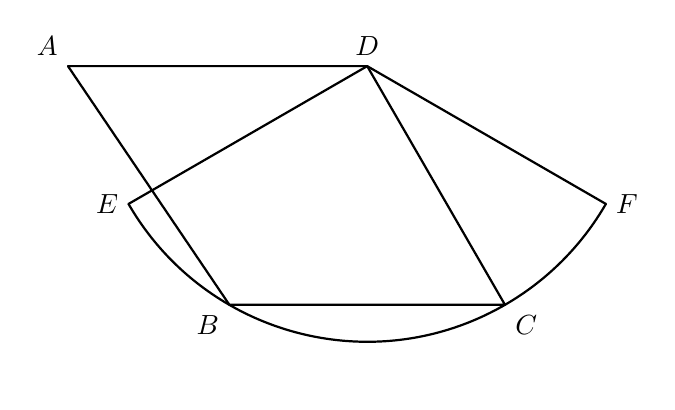
\begin{tikzpicture}[line cap=round, line join=round, >=stealth, x=1cm, y=1cm, thick]

    % --- 1. 定义几何参数 ---
    % 以D点为几何核心坐标系原点
    \coordinate (D) at (0,0);
    \def\R{3.5} % 定义半径 DE = DB = DC = DF

    % 定义各个点相对于D极坐标的角度
    \def\angE{210}
    \def\angB{240}
    \def\angC{300}
    \def\angF{330}

    % --- 2. 计算关键点坐标 ---
    \coordinate (E) at (\angE:\R);
    \coordinate (B) at (\angB:\R);
    \coordinate (C) at (\angC:\R);
    \coordinate (F) at (\angF:\R);

    % 根据梯形平行关系 AD // BC 确定 A 的位置
    % 视觉上 AD 为水平线，设置 A 的纵坐标与 D 相同 (y=0)
    \coordinate (A) at (-3.8, 0); 
    % D 保持在 (0,0)，所以 AD 在水平轴上

    % --- 3. 绘制图形边界 ---

    % 绘制扇形边缘和圆弧
    \draw (D) -- (E);
    \draw (D) -- (F);
    \draw (E) arc (\angE:\angF:\R);

    % 绘制梯形及内部连线
    \draw (A) -- (D) -- (C) -- (B) -- cycle;

    % --- 4. 标注文本节点 ---
    \node [above left] at (A) {$A$};
    \node [below left] at (B) {$B$};
    \node [below right] at (C) {$C$};
    \node [above] at (D) {$D$};
    \node [left] at (E) {$E$};
    \node [right] at (F) {$F$};

\end{tikzpicture}
\end{document}